\documentclass[conference]{IEEEtran}
\usepackage{amsmath,amssymb,amsfonts}
\usepackage{algorithmic}
\usepackage{graphicx}
\usepackage{textcomp}
\usepackage{xcolor}
\usepackage{biblatex}
\usepackage{titlesec}
\usepackage{float}
\usepackage{listings,xcolor}



\def\BibTeX{{\rm B\kern-.05em{\sc i\kern-.025em b}\kern-.08em
		T\kern-.1667em\lower.7ex\hbox{E}\kern-.125emX}}


\addbibresource{references.bib}

\begin{document}

	
\title{Speaker Voice Similarity Analysis and Evaluation}

	
\author{\IEEEauthorblockN{Carmel Gafa}
	\date{April 2025}
	
}

\maketitle

\begin{abstract}
This study investigates the effectiveness of a WavLM-based system in distinguishing between 285 different speakers from the ABI-1 dataset. \end{abstract}



\section{Introduction}

Speaker identification is the determination of a speaker's identity from a segment of their speech. It is crucial in applications such as personalized voice assistants, security systems, and partitioning audio streams according to each speaker's identity. Unlike speech recognition, which focuses on what is being said, speaker identification is concerned with who is speaking.

This task can effectively be approached as a downstream application of pre-trained self-supervised speech models, such as \texttt{Wav2Vec2}\cite{baevski2020wav2vec} or its enhanced variant \texttt{WavLM}\cite{chen2022wavlm}. These models are trained on large-scale unlabelled audio datasets to learn audio representations that capture phonetic and speaker-specific characteristics.

In this project, \texttt{WavLM-base-plus-sv}, a fine-tuned version of \texttt{WavLM} specialized for speaker verification, is used to extract speaker embeddings from audio samples. These embeddings are compared using cosine similarity to measure the similarity of two voice samples. This architecture enables a simple speaker identification pipeline without the need to train a model from scratch.


\section{Data preprocessing}

The Accents of the British Isles (ABI) Corpus represents 13 regional accents. Figure \ref{fig:img-abi-corpus-accents} shows how these accents are categorized into four broad accent groups; Scottish, Irish, Northern English, and Southern English. Each broad group is further split into its respective regional accents\cite{najafian2016improving}.

\begin{figure}[H]
	\centering
	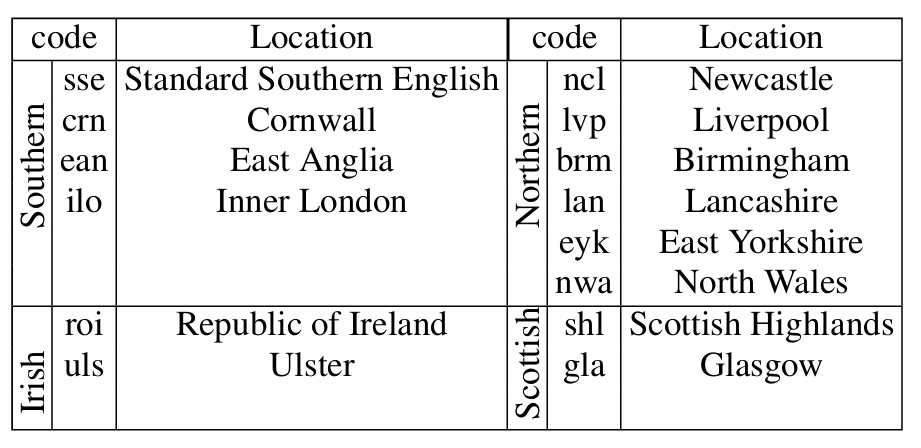
\includegraphics[width=0.7\linewidth]{img/img-abi-corpus-accents}
	\caption{Accents represented by the ABI Corpus\cite{najafian2016improving}.}
	\label{fig:img-abi-corpus-accents}
\end{figure}

The corpus includes 285 subjects, with speech collected from individuals who have lived in each regional accent area since birth. Each of the 285 subjects read the same three short passages. These are short paragraphs forming the 'sailor passage', with lengths of 92, 92, and 107 words with average durations of 43.2, 48.1, and 53.4 seconds, respectively\cite{najafian2016improving}.

The sources do not explicitly describe the recording conditions of the ABI corpus, however, it is mentioned that the speakers were selected by a phonetician, suggesting an effort for a standard quality recording for at least that accent\cite{najafian2016improving}.

\subsection{Signal resampling}

Audio signals depend on two main parameters

\begin{itemize}
	\item number of channels $C$, that is $1$ for mono and $2$ for stereo.
	\item number of samples $T = t \times f_s$; that in turn depends on the
	\begin{itemize}
		\item duration $t$ of the audio in seconds.
		\item sampling rate $f_s$ (e.g. 48,000 Hz).
	\end{itemize}
	
\end{itemize}

For a mono signal, that is common in these applications, a vector representing the utterance is available for processing,  $\mathbf{x}_{\text{raw}} \in \mathbb{R}^{1 \times T}$ in this way.


The model by Microsoft that we are using in this example expects a signal rate of 16,000 Hz, and it is therefore necessary to resample the signal to this frequency. The resampling step involves selecting a subset of samples from the original vector, so that the original sampling rate $f_s^{\text{raw}}$ becomes a lower one $f_s^{\text{target}}$. The down-sampling ratio in this case, $R = \frac{f_s^{\text{raw}}}{f_s^{\text{target}}} = 3$


Before reducing the number of samples, the high-frequency components from the original signals are removed, as they could cause aliasing. Aliasing occurs when frequencies above the new Nyquist frequency (which is one-half the new sampling rate) “fold back” into the signal, corrupting it. The Nyquist frequency after down-sampling becomes:

$$f_N^{\text{new}} = \frac{f_s^{\text{target}}}{2} = 8000~\text{Hz}$$

To remove the high frequency components, a low-pass filter is applied, generating a filtered signal, $\tilde{x}$

$$\tilde{x}[n] = x_{raw}[n] * h[n]$$

where $h[n]$ is the impulse response of a low-pass filter, typically a windowed \texttt{sinc} function:

$$h[n] = \text{sinc}\left(\frac{n}{R}\right) \cdot w[n]$$

Here, $w[n]$ is a window function (like Kaiser, Hamming, etc.) to localize the infinite \texttt{sinc} filter in time.

If, as an example, we consider this function:

\begin{align*}
	x_{raw} &=[x[0], x[1], x[2], x[3], x[4], x[5], x[6], x[7], x[8]]\\
		 	&=[2, 4, 6, 8, 10, 8, 6, 4, 2]
\end{align*}

and use the following windowed \texttt{sinc} filter (kernel)

\begin{align*}
	h &= [h[0],\ h[1],\ h[2]]\\
	  &= [0.2,\ 0.6,\ 0.2]
\end{align*}

We slide the kernel over the signal and compute:

$$\tilde{x}[n] = \sum_{k=0}^{2} x[n + k] \cdot h[k]$$

So that the first two samples of the filtered signal becomes

\begin{align*}
	\tilde{x}[0]	&= 0.2 \cdot x[0] + 0.6 \cdot x[1] + 0.2 \cdot x[2] \\
					&= 0.2\cdot2 + 0.6\cdot4 + 0.2\cdot6 \\
					&= 0.4 + 2.4 + 1.2 \\
					&= 4.0\\
	\tilde{x}[1] 	&= 0.2 \cdot x[1] + 0.6 \cdot x[2] + 0.2 \cdot x[3] \\
					&= 0.2\cdot4 + 0.6\cdot6 + 0.2\cdot8 \\
					&= 0.8 + 3.6 + 1.6 \\
					&= 6.0
\end{align*}

Once the signal is filtered, we can keep every $R^\text{th}$ sample and discard the rest (decimation), or alternatively, apply interpolation to produce a smoother, resampled signal at the desired rate.

$$x_{\downarrow R}[n] = x[Rn]$$

So that, for example,

$$x_{\downarrow 3}[n] = x[0], x[3], x[6], x[9], \dots$$







\begin{figure}[H]
	\centering
	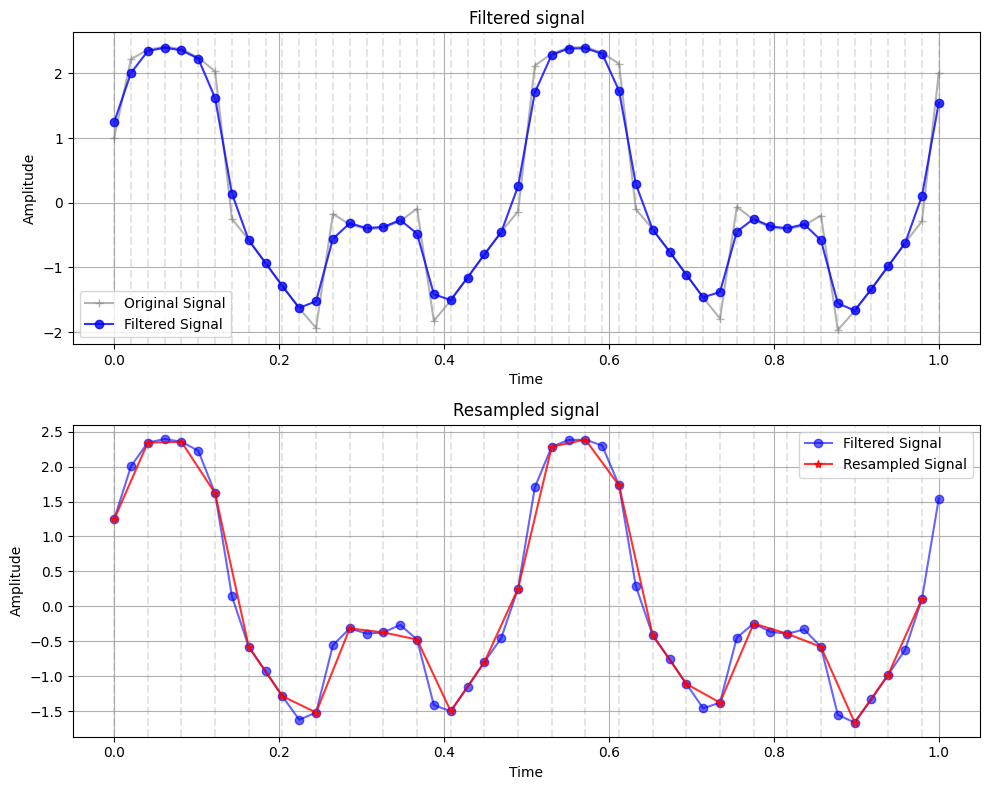
\includegraphics[width=0.9\linewidth]{img/img-resampling}
	\caption{}
	\label{fig:img-resampling}
\end{figure}




\section{Methodology}


\begin{figure}[H]
	\centering
	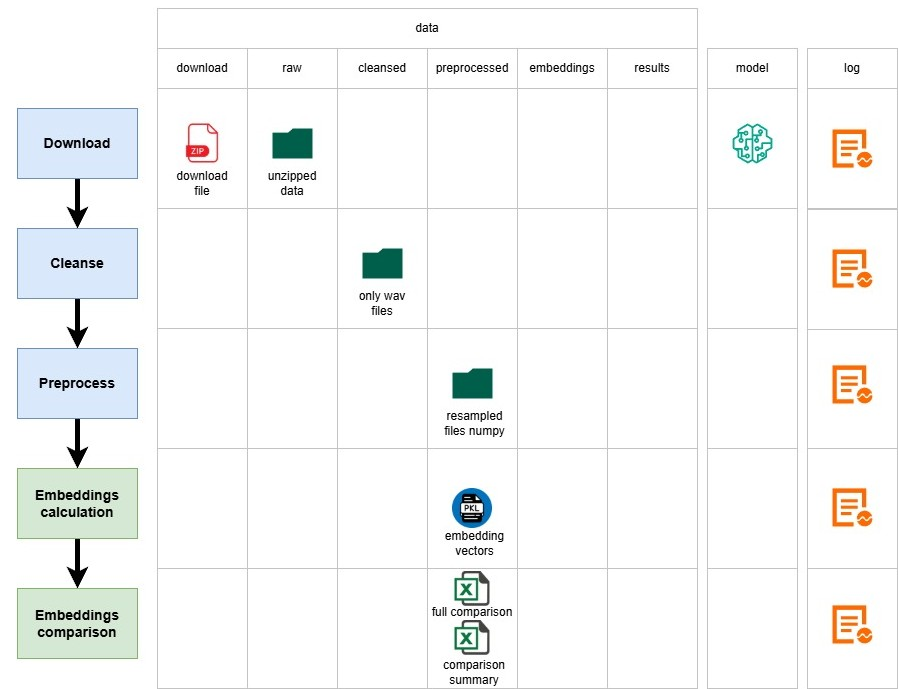
\includegraphics[width=1\linewidth]{img/img-pipeline}
	\caption{}
	\label{fig:img-pipeline}
\end{figure}

\section{Evaluation and results}


\section{Analysis and discussion}

\section{Conclusion and future work}




\section*{Generative AI}

\printbibliography


	
\end{document}
